\section{Domain-agnostic Results} \label{sec:results_domain_agnostic}

We present our domain-agnostic studies on the \textit{spacing} and \textit{placing} of duplicates in LLM training. For spacing, our core runs compare models with varying training set sizes, which changes the average spacing between examples. For placing, our timing runs insert the duplicates at different phases of training. Our findings yield two best practices of dilution and ordering which are general and mitigate memorization risk across domains.

\begin{figure}[h]
    \centering
    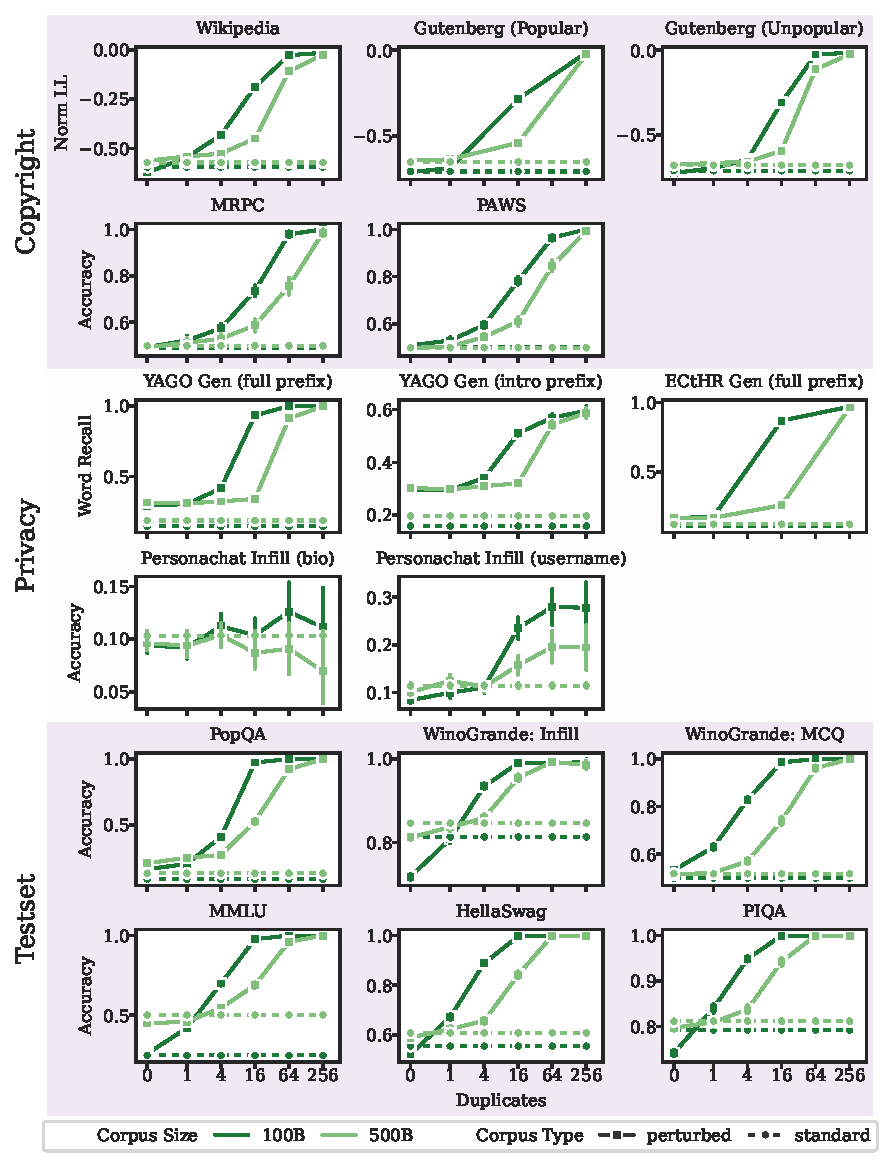
\includegraphics[width=\textwidth]{figures/dilution/dilution-hubble_8b.pdf}
    % \vspace{-4ex}
    \caption{\textbf{Memorization of sensitive data can be diluted by training on larger corpora.} We report the base evaluations on a subset of tasks for the core 8B models trained on 100B and 500B tokens. The core runs are described in \S\ref{sec:models} and evaluations are described in \S\ref{sec:evaluations}. For the same duplicate level, memorization is weaker for the model trained on 500B tokens compared to 100B. Figure \ref{fig:model_scale-dclm_500b} compares these trends against the 1B models, and larger models memorize at lower duplications. These experiments represent multiple interventions in one training run, and Figure \ref{fig:interference-full} plots these results for our interference models, which confirm minimal interference across domains.}
    \label{fig:dilution-hubble_8b}
\end{figure}
\clearpage

\textbf{Diluting sensitive data by training on larger corpora reduces memorization risks.} Figure \ref{fig:dilution-hubble_8b} plots the memorization evaluations for the perturbed 8B models trained on either 100B or 500B tokens. Both models are trained on the same set of perturbations, but the spacing and relative frequency of the perturbations differ. When trained on more tokens, the model's memorization on nearly all tasks in all domains increases slower with respect to frequency. This generalizes the result of \citet{bordt2025how}, which showed that scaling the training corpus reduces the effect of test set contamination. These findings suggest a simple best practice to address memorization risks broadly: sensitive data can be \textit{diluted} by training on larger corpora and is complementary to the best practice of deduplication \citep[recommended in][]{pmlr-v162-kandpal22a,lee-etal-2022-deduplicating}.

% cite forgetting papers
\textbf{Ordering sensitive data to appear early in training reduces memorization risks.} We present a selection of results for the timing runs in Figure \ref{fig:injectrange-main} and the full set of results in Figure \ref{fig:injectrange-full}. When perturbations are inserted in only the first quarter of training, the final model does not memorize the data. From Figure \ref{fig:checkpoint-forgetting-curves}, the intermediate checkpoints show that if the model does not receive continued exposures to duplicates, the model can forget the perturbations, which provides a form of privacy \citep{jagielski2023measuring,chang2024large}. When all perturbations are inserted in the last quarter of training, more data is memorized and extractable than the regular perturbed model. This is consistent with \cite{more2025realisticextractionattacksadversarial}, which finds that data at the end of training is more likely to be extractable. This suggests a second best practice to address memorization risks: sensitive data can be \textit{ordered} to appear early in training. 

\textbf{Larger models memorize at lower duplications.} Figure~\ref{fig:model_scale-dclm_500b} compares the memorization strength of both the 1B and 8B parameter models trained on the 500B token corpus. Consistent with prior work \citep{tirumala2022memorization}, the 8B model shows higher memorization across all tasks at the same duplication level, and memorization is measurable with fewer duplicates. Increasing the model size increases memorization risk, so practitioners will need to balance the effects of model scaling with other mitigation strategies such as dilution or ordering.

% \textbf{The concentration of perturbations affects the memorization.} Two sets of results, first comparing concentrations starting at 0 (denser is faster memorization). And then 2 concentrations ending at 50 (sparser is slower decay). And then the final memorization strength for checkpoints ending at 100 (denser is stronger).
% This finding supports the \textit{learnability threshold} proposed by \citet{}: models will not retain a fact if it is not re-encountered in a certain number of training steps.

% \textbf{Pre-training on more tokens consistently dilutes memorization.} Figure \ref{}

% \subsection{Recommendations}
% this will go to the appendix
% Memorization risks of LLMs will likely be managed through a body of soft law, which are non-binding rules, guidelines, and best practices. While such practices lack the backing of legislation, they often derive legitimacy from judicial or executive authority \citep[e.g. when a judge determines the legality of a new technology based on whether its deployment adheres to best practices;][]{hagemann2018soft}, and can gain industry adoption. Besides the outputs of LLMs and safeguards, \cite{wei_2025_interrogating} point out that the structural design choices of LLMs may be scrutinized by judges or regulators when assessing copyright risk, and major commercial models, such as Gemini, already emphasize measurements of memorization in their public documentation \citep{team2024gemini, apertus2024}.
% A well-established best practice is deduplication, which reduces the likelihood of memorization by removing repeated examples from the training corpus \citep{lee-etal-2022-deduplicating, hans2024be}. Yet deduplication has limits: not all sensitive information can be identified or eliminated, and other factors such as the distribution of examples across training time can also affect memorization \citep{tirumala2022memorization, pmlr-v162-kandpal22a, DBLP:conf/iclr/CarliniIJLTZ23, chang2024large, more2025realisticextractionattacksadversarial}. Our core experiments establish a second, complementary best practice: dilution. By training on larger corpora, models become more tolerant to insertions of sensitive information, reducing their relative prominence. This effect has also been observed from a forgetting perspective \citep{bordt2025how}. Together, deduplication and dilution expand the technical toolkit available for mitigating memorization risk.

% \subsection{Temporal effects}
% - inject range memorization
% - checkpoints (for inject range)
% - different visualizations?

% For the original perturbed model, the perturbation data was injected uniformly randomly throughout training. We train six additional models to measure the effect of the number of training steps before and after exposure to the perturbation data on the strength of memorization. These models have 1B parameter models and are trained on 100B tokens, where the perturbation data is injected in a specific range of batches: (0\%, 50\%), (50\%, 100\%), (0\%, 25\%), (25\%, 50\%), (50\%, 75\%), (75\%, 100\%). The percentage refers to the progress in the overall training; e.g. (50\%, 100\%) means batches in the second half of training.

\begin{figure}[t]
    \centering
    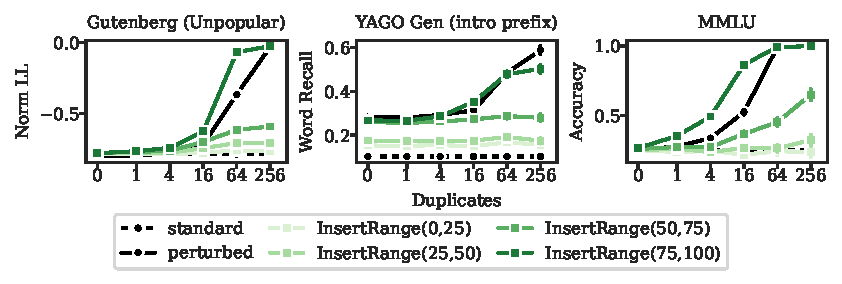
\includegraphics[width=\textwidth]{figures/injectrange/injectrange-main.pdf}
    \vspace{-4ex}
    \caption{\textbf{Sensitive data can be forgotten without continued exposure.} We report the performance of the Timing runs (1B models trained on 100B tokens, described in \S\ref{sec:models}) where perturbations are inserted in different phases of pretraining (tuples denote the range of pretraining where texts are inserted). For reference, the standard and perturbed 1B parameter models are also plotted.}
    \label{fig:injectrange-main}
\end{figure}

% \todo{Nitya}{Add discussion on intermediate checkpoint analysis}

% \subsection{Interference}

%\begin{figure}
%    \centering
%    \includegraphics[width=\textwidth]{figures/interference/interference-main.pdf}
%    \caption{\textbf{The perturbed model matches the behavior of domain-specific models on the respective set of evaluations.} The perturbed model matches the \texttt{copyright\_only} model in memorizing the unpopular Gutenberg passages, \texttt{privacy\_only} model in generating memorized PII from biographies, and \texttt{testset\_only} model in memorizing MMLU questions. This figure contains a subset of the evaluations (refer to Figure\ref{fig:interference-full} for all evaluations).}
%    \label{fig:interference-main}
%\end{figure}

% As discussed in \S~\ref{sec:models},
\textbf{Perturbations from different domains minimally interfere with each other.} Our perturbed models are the product of many interventions in a single training run. If the perturbations interfere with each other (e.g., a highly duplicated example in a test set affects the memorization of a paraphrase), that would undermine the validity of our analyses. Although exhaustively characterizing such interference \citep[as in][]{ilyas_datamodels_2022} would be impractical, we perform a check by training three 1B models each containing perturbations from only a single risk domain. As shown in Figure~\ref{fig:interference-full}), the behavior of the core perturbed model matches every single-domain model on the corresponding domain. These suggest that our aggregate, domain-level findings have minimal interference.

\section{Domain-specific Results} \label{sec:results_domain_specific}

The perturbation data in \textsc{Hubble} is designed to enable a broad range of experimentation. In this section, we present tailored analyses for the specific data types in each domain.

\subsection{Copyright}

\textbf{Whether an LLM is considered to memorize depends on the metric.} In Figure \ref{fig:copyright-passages}, we additionally evaluate $k$-eidetic memorization \cite[introduced in][]{DBLP:conf/iclr/CarliniIJLTZ23} and the ROUGE-L metric on the passages in the copyright domain (details in Appendix \ref{app:copyright_specific_results}).  While loss can show statistically significant differences in memorization at lower duplicate counts, the $k$-eidetic metric does not. This can be seen for Wikipedia passages at 4 duplicates, where loss shows significant differences for the 8B, 100B model, but $k$-eidetic memorization does not, and differences only start to show at 16 duplicates.  For copyright debates, this means that the choice of metric affects the interpretation of a memorization analysis, and numerical measures are unlikely to be useful on their own.

\textbf{Popular and unpopular books are memorized similarly by the 1B model, with only minor differences for the 8B model.} Based on the data density hypothesis \citep{kirchenbauer2024lmd}, we expected popular books from Gutenberg would be memorized better than unpopular books, as popular books are more likely to be discussed in the pretraining corpus. In Figure \ref{fig:model_scale-dclm_500b}, At the 1B parameter scale, there is no noticeable difference, and at the 8B parameter scale, there is only a slight increase in the generative extraction of passages from popular books compared to unpopular books. The 8B parameter models trained on 100B and 500B tokens both assign a slightly higher likelihood to passages from the popular books. While we find little difference for popular books using basic evaluations, more sensitive methods may reveal subtler forms of memorization.

% Define color boxes for slots and attributes
\definecolor{slotgray}{gray}{0.9}
\definecolor{attrpurple}{HTML}{E6E6FA} % light lavender

\newcommand{\slotlabel}[1]{\colorbox{gray!20}{\texttt{#1}}}
\newcommand{\slot}{\colorbox{slotgray}{\texttt{<candidate>}}}
\newcommand{\attr}[1]{\colorbox{attrpurple}{\texttt{#1}}}

\begin{table}[t]
\centering
\small
\caption{\textbf{Attack Definitions for YAGO.} PII attacks are listed below in increasing order of strength (fewer additional PII known to the attacker). Each attack corresponds to a different prompt, and we illustrate the attacker's query to infer the target's university using a sample biography from YAGO. The full prefix–full suffix attack is only compatible with infill attacks (loss-based choice) since generations cannot be conditioned on the suffix. Attack success rates are presented in Figure \ref{fig:privacy-yago}, and a breakdown of success rate by PII type is given in \ref{fig:privacy-yago-meta}.}
\label{tab:pii_attack_definition}
\begin{tabularx}{\textwidth}{c c >{\raggedright\arraybackslash}X}
\toprule
\multicolumn{3}{>{\raggedright\arraybackslash\hsize=\textwidth}X}{
\textbf{Sample YAGO Biography (templated slots shaded purple)}%
}\\
\midrule
\multicolumn{3}{>{\raggedright\arraybackslash\hsize=\textwidth}X}{
\texttt{%
\attr{Dora Sloan} is from \attr{the United States}. %
\attr{Dora} was born in \attr{Phoenix, Arizona}. %
\attr{Dora} is an alumni of \attr{St. John's College}. %
\attr{Dora} was born on \attr{May 15, 1968}. %
\attr{Dora} receives email at \attr{dora@gmail.com}. %
\attr{Dora} is a \attr{competitive diver}. %
\attr{Dora} has the unique identifier \attr{4dc0969af29a4324bf5746c50f7209a2}.%
}
}\\
\toprule
\textbf{Prompt Format} & \textbf{Compatible Attack} & \textbf{Example Query (suffix underlined)} \\
\midrule
full prefix–full suffix & Infill &
\texttt{Dora Sloan is from the United States. Dora was born in Phoenix, Arizona. Dora is an alumni of }\underline{\slot\texttt{. Dora was born on}} ~~~~ \underline{\texttt{May 15, 1968. Dora receives email at}} ~~~~ \underline{\texttt{dora@gmail.com. Dora is a competitive diver.}} \underline{\texttt{Dora has the unique identifier}} \underline{\texttt{4dc0969af29a4324bf5746c50f7209a2.}}\\
\midrule
full prefix & Infill, Gen &
\texttt{Dora Sloan is from the United States. Dora was born in Phoenix, Arizona. Dora is an alumni of }\underline{\slot\texttt{.}}\\
\midrule
intro prefix & Infill, Gen &
\texttt{Dora Sloan is from the United States. Dora is an alumni of }\underline{\slot\texttt{.}}\\
\midrule
name only & Infill, Gen &
\texttt{Dora Sloan is an alumni of }\underline{\slot\texttt{.}}\\
\bottomrule
\end{tabularx}
\end{table}

\subsection{Privacy}

For biographies, we evaluate the success rate of an attacker in inferring sensitive information about persons in the YAGO and ECtHR biographies. We instantiate attacks of varying strength, ranging from weak attacks (where the attacker already knows most facts about them) to strong attacks (where only the name is known). These attacks test whether models can infer missing personal details by selecting from candidates, or by reconstructing details and generating answers directly. Different attacks correspond to different prompts and Table \ref{tab:pii_attack_definition} visualizes them for YAGO. YAGO results are reported in Figure \ref{fig:privacy-yago}, and the breakdown by PII type is given in Figure \ref{fig:privacy-yago-meta}. Further details and results on ECtHR are in Appendix~\ref{app:direct_pii_leakage}. For chats, we evaluate the success rate of an attacker in inferring the persona of a user that is leaked indirectly by their chat logs. The evaluation formats are described in Table \ref{tab:chat_attack_definition} and results on Personachat are presented in Figure \ref{fig:privacy-personachat}.

% For biographies, we not only evaluate the memorization of the biographies but also whether sensitive information can be inferred about the fictional people. For direct memorization, we report the loss assigned by the model to the inserted biography. To evaluate the ease of PII reconstruction, we instantiate attacks with varying strength. \textbf{Weak attacks} assume that the attacker already knows PII about the person of interest and is seeking a few missing facts. \textbf{Strong attacks} assume that the attacker knows less sensitive information about the person of interest, with our strongest attacks assuming that the attacker only knows the name. We instantiate \textbf{loss-based choice attacks} where the attacker has narrowed down the possible values of the missing PII. We frame the attack as MCQ problems and check which candidate answer has the highest likelihood when plugged into the blank. When the attacker has no way to deduce the set of candidate answers, they have to use \textbf{generative attacks} where the model is prompted to fill in the blank. We evaluate generative attack with either \textit{Word Recall}, which scores if the answer entity occurs anywhere in the generated response, or \textit{Prefix Match}, which scores whether the model generation starts with the answer entity. Table \ref{tab:pii_attack_definition} lists the attacks that we instantiate. The synthetic YAGO biographies allow us to instantiate each of the attacks listed in the table. We can only instantiate the \textit{full prefix, generative} attack for ECtHR since the entity types are not clearly defined (e.g., dates can refer to birth dates or event dates) and not all entity types are always present in the biography. Figures \ref{fig:privacy-ecthr} and \ref{fig:privacy-yago} report attack success rates on ECtHR and YAGO perturbation sets, respectively. Figure \ref{fig:privacy-yago-meta} provides a breakdown by PII type for reconstruction attacks on YAGO biographies (rows are arranged in the order that the PII type occurs in the biography).

% \textbf{Privacy.} In Appendix \ref{app:privacy_specific_results}, we study the reconstruction of PII in YAGO biographies. We find that the more pieces of auxiliary information the attacker has access to, the higher the success rate of reconstruction for a given PII in the biography. For the paraphrased models, which were trained on paraphrased biographies, PII reconstruction attacks remains successful. This means the paraphrased model has not just memorized a fixed string, but generalizes to unseen queries for the PII and this knowledge is retrievable \citep[similar to the retrievability observed in][]{allen-zhu_physics_2024}. Personachat also shows the model's ability to retrieve memorized information, and models can infer a user's persona based on the memorized chat logs (although the accuracy is low).

\textbf{The more auxiliary information the attacker has access to, the higher the success rate.} For both ECtHR (Fig \ref{fig:privacy-ecthr}) and YAGO (Fig \ref{fig:privacy-yago}), the attacks with the most auxiliary information are the most effective in inferring PIIs with high accuracy. Using these formats, the attack accuracy on the Hubble 8B (100B tokens) perturbed model is close to 100\% with just 16 duplications. When provided less auxiliary information (e.g. name only) the accuracy of inference decreases significantly.

\textbf{Memorization research needs to account for variation across PII data types.} By comparing attack success across PII types \citep{lukas2023analyzing}, we find that certain attributes such as occupation, email, and UUID are memorized differently from others. Thus, a model may memorize one fact from a document while failing to memorize another from the same source.

\paragraph{Inference of indirect information is difficult but possible.} The details of our analysis on PersonaChat is in Appendix \ref{app:indirect_pii_extraction}. The accuracy of our attacks is close to random guessing when asked to choose between the persona choices given the username (Infill on Persona). While the Hubble models memorize the chat logs for the user, they do not directly assign higher likelihoods to the correct underlying persona. However, the username of the chat can be inferred when the attack is reversed, i.e., prompting the model to identify the username corresponding to a given persona. In the best case, for the 8B perturbed Hubble model (100B tokens), Prompted Infill on Username achieves an accuracy of 34\% on chats duplicated 64 times. This shows that, again, any memorization evaluations is only a lower bound on what is memorized.

\textbf{PII can still be inferred from paraphrased biographies.} In Appendix \ref{app:paraphrase_results}, we trained a `paraphrase' model with different paraphrases rather than exact duplicates of the biographies. The high accuracy of PII recontruction and inference indicates the paraphrase model has not just memorized a fixed string; instead, it generalizes to unseen queries for the PII, and this knowledge remains retrievable \citep[similar to the retrievability observed in][]{allen-zhu_physics_2024}.
The accuracy of strong name-only attacks is higher on the 8B-parameter paraphrase model than on the original perturbed model at high duplication levels, indicating that models trained on paraphrases develop stronger semantic memory than the verbatim memory formed from training on exact duplicates.
Personachat also shows the model's ability to retrieve memorized information in new contexts, and models can infer a user's persona based on the memorized chat logs (although the accuracy is low).

\subsection{Test Set Contamination}

% pretraining on test set examples, doesn't help you generalize on test sets. 
\textbf{Models begin to memorize test set examples with as few as one duplicate, but generalization to unseen examples is unpredictable.} From Figure \ref{fig:testset-set1}, we see that the Hubble perturbed models trained on 100B tokens show an increase in accuracy on PopQA, HellaSwag, and PIQA with just 1 instance of contamination.
However, memorizing test set examples does not translate into generalization on that task: perturbed models show no improvement over standard models when trained on contaminated tasks (reflected in model performance on 0 duplicates), aside from small improvements on PopQA and under certain settings of HellaSwag. In fact, model performance on unseen examples degrades for WinoGrande and a few settings of HellaSwag.
For WinoGrande (see Figure \ref{fig:testset-wg}), we find that perturbed models achieve worse accuracy on minimal pairs of contaminated examples than unseen examples. Further analysis and details are presented in Appendix \ref{app:testset_specific_results}.
Likewise, the paraphrased model fails to answer MMLU questions which were contaminated with paraphrases of that question. We hypothesize that pretraining on a handful of contaminated test examples is not enough to generalize on the task, leading only to memorization.

\paragraph{For WinoGrande, models do not generalize across formats and have worse accuracy on contaminated examples in a new format than on unseen examples.} We inserted two variants of WinoGrande, one in the standard infill (cloze) format, and another in the MCQ format, where options are presented with the question and the model has to generate the correct option. In Figure \ref{fig:testset-wg}, we report the model accuracy when the test time format does not match the inserted format. For examples inserted with the MCQ format, when tested on the infill format, the perturbed model accuracy even decreases with increased duplication.

% Our perturbed models represent multiple interventions from multiple experiments. A validity concern is that many perturbations in the same training run could cause interference effects (e.g. if two perturbations were close duplicates of each other), making it unclear whether results reflect the intended perturbation or unexpected interactions. In general, checking for all interferences is difficult and requires advanced methods to determine example influence \citep{ilyas_datamodels_2022}.
% We train three 1B parameter models on three different corpora each containing perturbations from only one domain. We highlight a subset of our findings in Figure \ref{fig:interference-main} (see Figure \ref{fig:interference-full} for the remaining evaluations). Our evaluations establish that the core perturbed model (trained on perturbations from all domains) matches the behavior of a model trained on perturbations from just the copyright domain (\texttt{copyright\_only}) on the copyright evaluations. Corresponding findings hold for the \texttt{privacy\_only} and \texttt{testset\_only} ablations. Thus, our core perturbed models remain valid for studying each domain individually, behaving as if they were trained on that domain alone despite joint training.

% Test set contamination.  However, this memorization does not translate into broader generalization: performance on unseen examples shows only marginal gains (e.g., PopQA, HellaSwag), and paraphrased training examples do not help the model answer the originals (Figure \ref{fig:paraphrase-full}). In other words, pretraining on contaminated test set examples leads to memorization of those items rather than meaningful generalization.
% We also identify a case on Winogrande where exposure to some examples makes the model worse at generalizing to unseen examples, as the dataset includes minimally contrasting examples with different answers (see Figure \ref{fig:testset-wg}).

% We reiterate that our evaluations are designed to serve as lower bounds, i.e., there may exist other formulations of prompts and tasks that elicit more copyright violations, leak sensitive information, and achieve higher leaderboard scores with the same set of models.

% \section{Experimental Results}

% main paper results are general
% look in the appendix for results that are more specific to certain areas

% in the first part, we first analyze general memorization results.
% in the second part, we look at specific perturbation while yields interesting observations in specific domains
% This section is organized in two parts. First, we  present our domain-agnostic studies on the \textit{spacing} and \textit{placing} of duplicates in LLM training. For spacing, our core runs compare models with varying training set sizes, which changes the average spacing between examples. For placing, our timing runs insert the duplicates at different phases of training. Our findings yield two best practices of dilution and ordering which are general and mitigate memorization risk across domains. In the second part, we present our domain-specific studies, where we analyze specific perturbations in \textsc{Hubble} to yield a rich set of observations for the domains of copyright, privacy, and test set contamination.

% This section first presents our findings on the \textit{spacing} and \textit{placing} of duplicates in LLM training. Since our perturbations are randomly inserted throughout the training process, increasing the size of the training data increases the average spacing between duplicates. For spacing, our core runs show that increasing the total amount of training data, which increases the average spacing between examples, reduces memorization. For placing, our timing runs insert the duplicates at different phases of training, and our findings show that memorization is strongest when duplicates appear closer to the end of training. This leads to two best practices which are domain-agnostic: dilution and ordering.
% An intuition from \cite{chang2024large} is that the memorization of an example is peaky, spiking when a duplicate is encountered and decaying afterward.
% Besides our results on general memorization risk, we include a variety of domain-specific experiments in Appendix \ref{app:domain_results}. We simulate a number 